\documentclass{article}

\usepackage[a4paper, total={6.5in, 11in}]{geometry}
\usepackage{graphicx}
\graphicspath{{titech/CSC.T527.FaultTolerantDistributedAlgorithm/}}

\usepackage{latex/common}

\title{FTDA 2021 - Homework 2}
\author{Sixue Wang\\Tokyo Institute of Technology}

\begin{document}

\maketitle

\section*{Question 1}
The algorithm has two stage:
\begin{itemize}
  \item The purpose of each process in the first stage is to find other $\lceil (N+1)/2 \rceil - 1$ alive processes. The easiest way is to broadcast identifier(process number) to all others, and then wait for other $\lceil (N+1)/2 \rceil - 1$ processes'.
  \item The purpose of each process in the second stage is to construct a clique which has $\lceil (N+1)/2 \rceil$ processes at least. In order to achieve this goal, each process continuously sends the following message 1) initial value; 2) all known processes' identifier; to all known processes. When a new process is recognized, it's also need to send the message to this process. It will stop until all known processes' messages are received and there is no more new processes.
\end{itemize}

\section*{Question 2}
\begin{itemize}
  \item Termination: At the first stage, each process can receive $\lceil (N+1)/2 \rceil - 1$ responses because a majority of the processes$(\geq \lceil (N+1)/2 \rceil)$ are alive initially. At the second stage, no processes will die at this time, so each process can receive the responses from known processes. Therefore, neither the first nor the second stage will be blocked, so the final decision will be made.
  \item Validity: All processes make decision among the initial values from alive processes, so the decision is valid.
  \item Agreement: After the first stage, every process knows $\lceil (N+1)/2 \rceil$ including itself. Then the transitive $G^+$ has $\lceil (N+1)/2 \rceil$ processes at least. If a process is not in $G^+$ then we treat it as a faulty process.
\end{itemize}

\section*{Question 3}
Case 1: \\
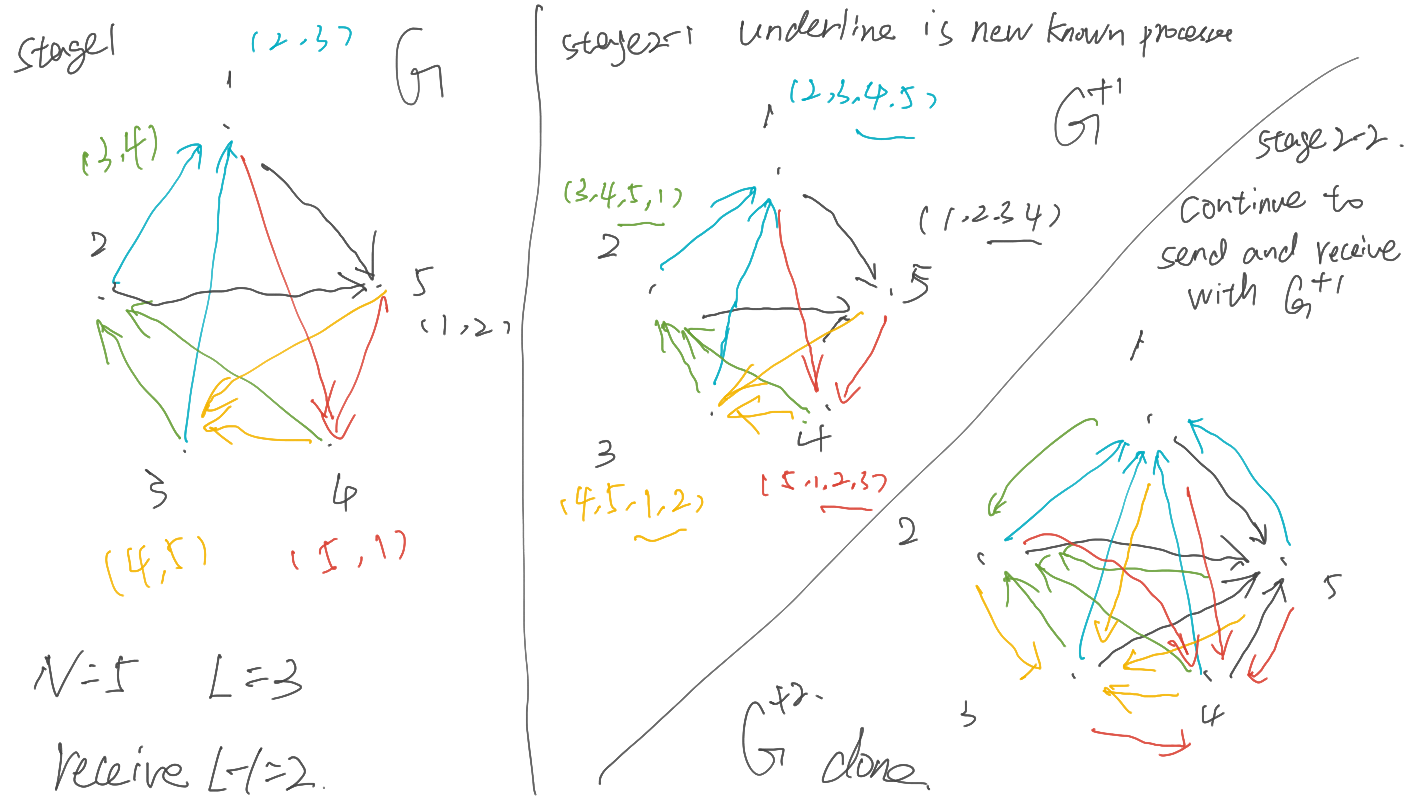
\includegraphics[width=\textwidth]{hw2_1}
Case 2: \\
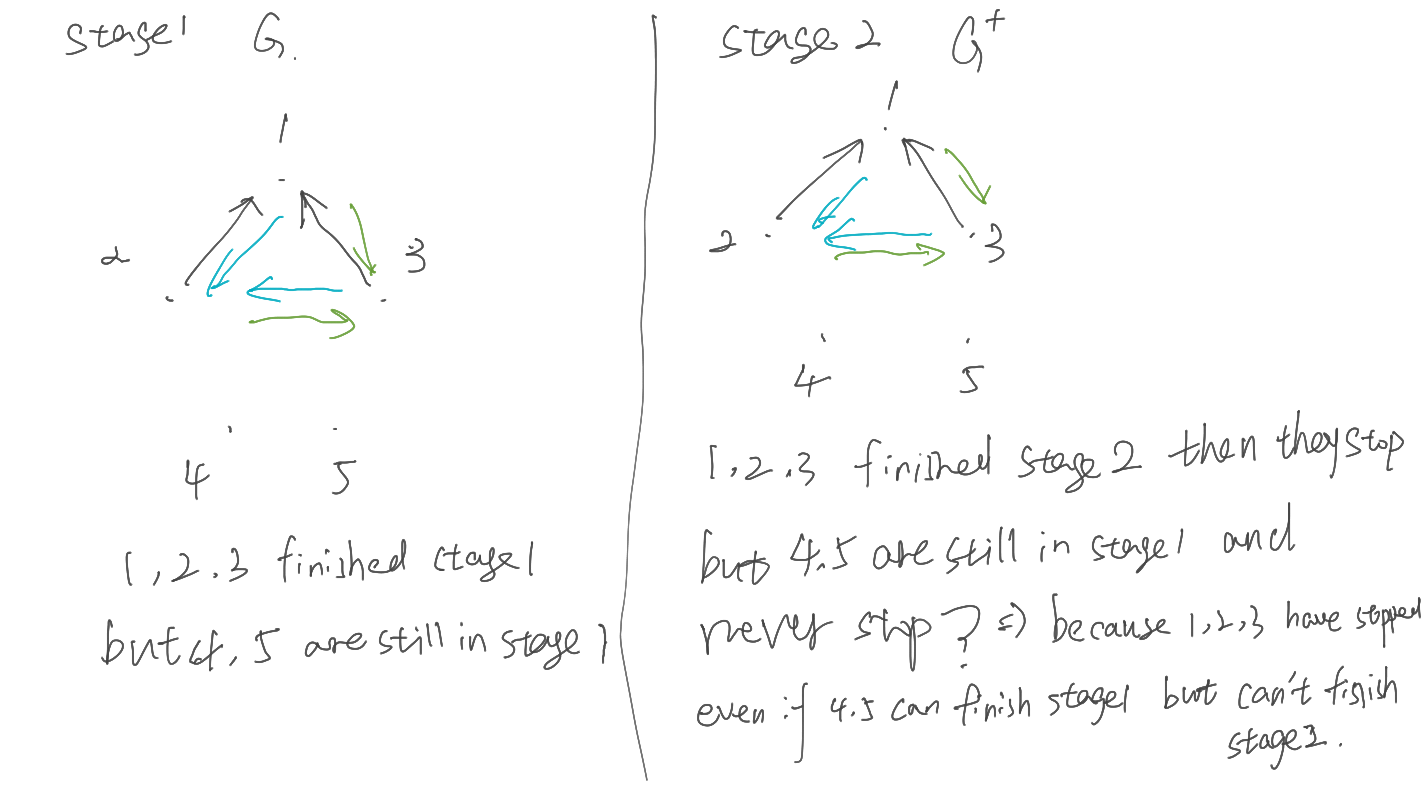
\includegraphics[width=\textwidth]{hw2_2}

\section*{Question 4}
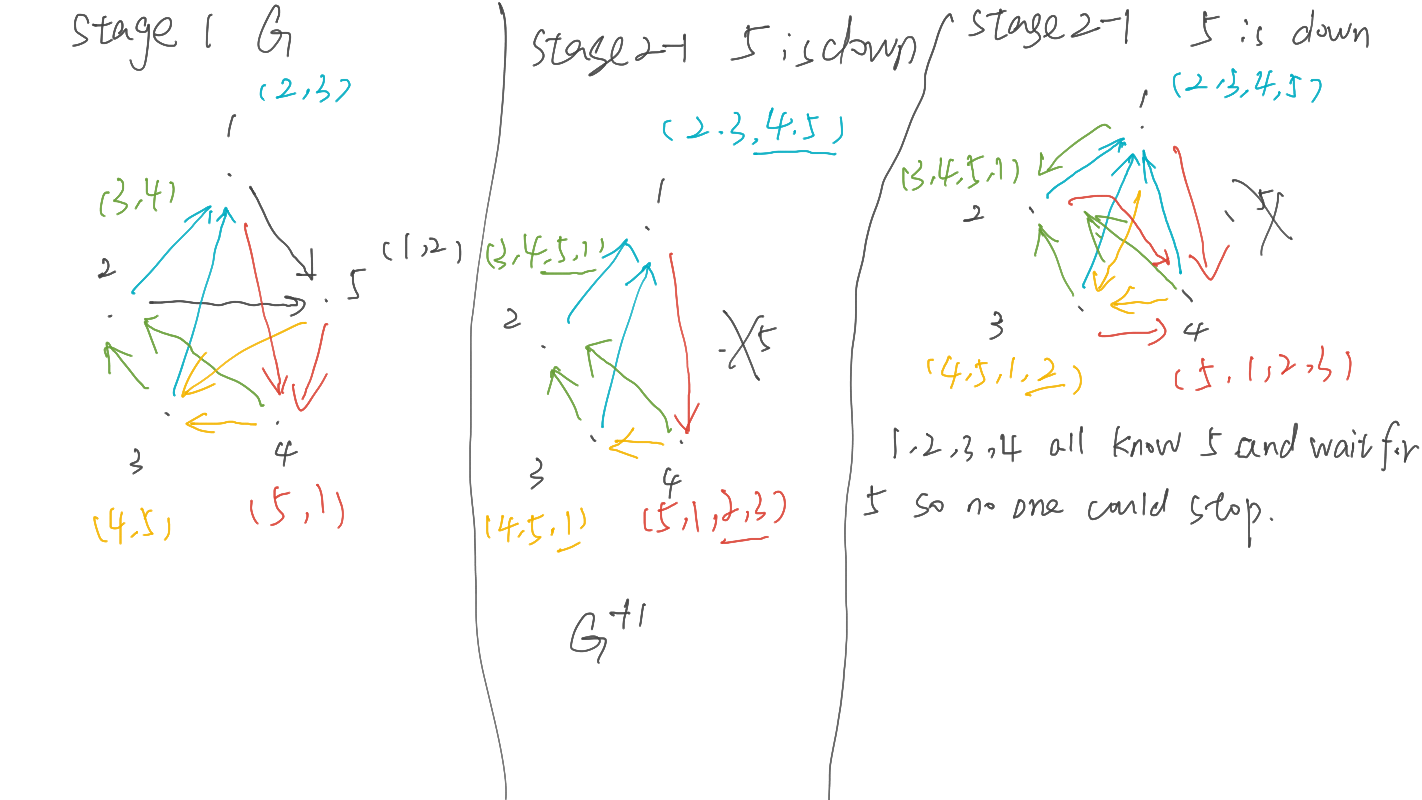
\includegraphics[width=\textwidth]{hw2_3}

\end{document}
